\documentclass[pdf]{beamer}
\usepackage[utf8]{inputenc}
\usepackage{ragged2e}
\setbeamertemplate{navigation symbols}{} % Ocultar iconitos abajo
\usepackage{xcolor}
\useoutertheme{infolines}{\title{}}
\usetheme{Warsaw}
\usepackage{hyperref}
\usepackage[T1]{fontenc}
\useinnertheme{rounded}

\title{Présentation de l'article : Massive MIMO Forward Link Analysis for Cellular Networks}
\author{Panongbene jean Mohamed Sawadogo}
\institute{Ecole Polytechnique - 3rd year of Ecole Polytechnique}
\date{10 January 2021}

\begin{document}

\frame{\titlepage}
\begin{frame}
\frametitle{Plan de Présentation }
\begin{enumerate}
	\item \hyperlink{Introduction}{Introduction}.
	\item \hyperlink{networkModeling}{Network Modeling}
	\item \hyperlink{conjugateBeamforming}{Conjugate Beamforming} 
	\item \hyperlink{spatialDistribution}{Spatial Distribution of $\rho_k$}
	\item \hyperlink{spatialsir}{Spatial SIR Distributions with fixed K}
	\item \hyperlink{spectralEfficiency}{Spectral Efficiency}
	\item \hyperlink{impactOfNoise}{Impact of Noise}
	\item \hyperlink{piloteContamination}{Pilot Contamination}
	\item \hyperlink{autredoc}{Géométrie stochastique et réseaux Massive MIMO}
\end{enumerate}
\end{frame}

\begin{frame}
\frametitle{Plan de Présentation }
\begin{enumerate}
	\item \hyperlink{Introduction}{Introduction}
\end{enumerate}
\end{frame}

\begin{frame}[label=Introduction]
\frametitle{Introduction}
\setbeamercovered{dynamic}
\transblindshorizontal
\begin{exampleblock}{Travail effectué :}
\justify
Cette présentation est un résumé explicative du travail qui a été effectué dans l'article scientifique \href{https://arxiv.org/pdf/1811.00110.pdf}{\color{blue}{Massive MIMO Forward Link Analysis
for Cellular Networks}} par le membre de l'IEEE {\color{blue}{Geordie Georg}} et les "Fellows" de l'IEEE {\color{blue}{Angel Lozano}} et {\color{blue}{Martin Haenggi}}.
\end{exampleblock}\pause
\begin{exampleblock}{Sujet étudié :}
\justify
Cet article présente des expressions analytiques du SIR(signal-to-interference-ratio) et de l'efficacité spectral du signal dans les réseaux macro-cellulaires avec formation de faisceau massive MIMO(massive MIMO conjugate beamforming) dans une configuration à la fois uniforme et dépendant du canal de la puissance.
Pour se faire, ils utilisent la puissance de la géométrie stochastique qui d’ailleurs a fait ces preuves dans des contextes non MIMO
\end{exampleblock}
\end{frame}

\begin{frame}
\frametitle{Plan de Présentation }
\begin{enumerate}
	\item \hyperlink{Introduction}{Introduction}
	\item \hyperlink{networkModeling}{Network Modeling}
\end{enumerate}
\end{frame}

\begin{frame}[label=networkModeling]
\frametitle{Network Modeling}
\setbeamercovered{dynamic}
\transblindshorizontal
\begin{exampleblock}{Modélisation à grande échelle :}
\justify
Remarque : chaque utilisateur est servi par la station de base(BS) à partir de laquelle il a le plus fort gain de canal à grande échelle.\\
Le gain de canal à grande échelle entre l'utilisateur k servi par la station de base p et la BS l est donné par :  
$$G_{l,(p,k)}=\frac{L_{ref}}{r_{l,( p,k)}^{\eta}}\chi_{l, (p,k)}$$
Où L$_{ref}$ est la perte de trajet à une unité de distance. Et ${r_{l,( p,k)}^{\eta}}$ est la distance entre l'utilisateur et la BS. $\chi_{l, (p,k)}$ est le coefficient d'ombrage vérifiant : $\mathbb{E}\left[\chi_{l, (p,k)}^{\delta}\right] < \infty$ with $\delta = \frac{2}{\eta}$
\end{exampleblock}
\end{frame}

\begin{frame}
\frametitle{Network Modeling}
\setbeamercovered{dynamic}
\transblindshorizontal
\begin{exampleblock}{Nombre d'utilisateur par BS :}
\justify
Pour chaque BS l, on note K$_l$ le nombre d'utilisateurs servi par cette station de base. Alors, il est démontré dans l'article que les $\left\lbrace K_l \right \rbrace_{l \in \mathbf{N}}$ suit une loi de poisson de paramètre $\tilde{K}=\mathbb{E}\left[K_l\right]$ borné par $N_a$ le nombre maximal d'utilisateur qu'une BS peut servir en même temps.\\
Ainsi, la probabilité que la station de base l serve k utilisateurs est donnée par : $$\mathbb{P}\left(K=k\right) = \frac{\tilde{K}^ke^{-\tilde{K}}}{k!}$$
\end{exampleblock}
\end{frame}

\begin{frame}
\frametitle{Plan de Présentation }
\begin{enumerate}
	\item \hyperlink{Introduction}{Introduction}
	\item \hyperlink{networkModeling}{Network Modeling}
	\item \hyperlink{conjugateBeamforming}{Conjugate Beamforming}
\end{enumerate}
\end{frame}

\begin{frame}[label=conjugateBeamforming]
\frametitle{Conjugate Beamforming}
\setbeamercovered{dynamic}
\transblindshorizontal
\begin{exampleblock}{Le signal transmit :}
\justify
Le signal transmit par la BS l est donnée par : $$x_l = \sum_{k=0}^{K_l-1}\sqrt{\frac{P_{l,k}}{N_a}}f_{l,k}s_{l,k}$$
O\'u P$_{l,k}$ est la puissance allouée au symbole $s_{l,k} \sim \mathcal{N}_{\mathbb{C}}\left(0,1\right)$ qui est précodé par $f_{l,k}$ qui est destiné au k ième utilisateur.
Nous avons : $\displaystyle \sum_{k=0}^{K_l-1}P_{l,k}=P= \mathbb{E}\left[\|x_l\|^2\right]$\\
Avec le beamforming et la contrainte de puissance moyenne, on peut écrire : 
$$f_{l,k} = \sqrt{N_a}\frac{\hat{h}_{l,(l,k)}}{\mathbb{E}\left[\|\hat{h}_{l,(l,k)}\|^2\right]}$$ avec $\hat{h}_{l,(l,k)}$ le canal estimé.
\end{exampleblock}
\end{frame}

\begin{frame}[label=conjugateBeamforming]
\frametitle{Conjugate Beamforming}
\setbeamercovered{dynamic}
\transblindshorizontal
\begin{exampleblock}{Signal-to-Interference Ratio(SIR) :}
\justify
En notant k un utilisateur deservi par une BS, alors le SIR associé à l'utilisateur k est donné : $$SIR_k = N_a \frac{P_k/P}{1+1/\rho_k}$$
O\'u P$_k$ est la puissance alloué à la tramission des symboles à l'utilisateur k et P est la puissance totale de la BS. The local-average SIR $\displaystyle \rho_k = \frac{G_{(k)}}{\sum_{l \neq 0}G_{l, (k)}}$ 
- Pour une allocation de puissance uniforme entre les utilisateurs  $P_k=\frac{P}{K}$, on a : $$SIR_{k}^{unif} = \frac{N_a/K}{1+1/\rho_k}$$
- On peut choisir d'allouer la même SIR moyenne local à tout les utilisateurs : $\displaystyle \rho_K = \frac{1}{\frac{1}{K}\sum_{k=0}^{K-1}\frac{1}{1/\rho_k}}$
\end{exampleblock}
\end{frame}

\begin{frame}[label=conjugateBeamforming]
\frametitle{Conjugate Beamforming}
\setbeamercovered{dynamic}
\transblindshorizontal
\begin{exampleblock}{Signal-to-Interference Ratio(SIR) :}
\justify
Dans ce cas on a : $$SIR_{k}^{eq} = \frac{N_a/K}{1+1/\rho_K}$$
\end{exampleblock}
Ces formules nous donnent le SIR pour les gains de liaisons à grande échelle données. 
\end{frame}


\begin{frame}
\frametitle{Plan de Présentation }
\begin{enumerate}
	\item \hyperlink{Introduction}{Introduction}
	\item \hyperlink{networkModeling}{Network Modeling}
	\item \hyperlink{conjugateBeamforming}{Conjugate Beamforming}
	\item \hyperlink{spatialDistribution}{Spatial Distribution of $\rho_k$}
\end{enumerate}
\end{frame}

\begin{frame}[label=spatialDistribution]
\frametitle{Spatial Distribution of $\rho_k$}
\setbeamercovered{dynamic}
\transblindshorizontal
Dans cette partie, nous définirons le SIR en éliminant les hypothèses faites sur les gains. Ainsi, les valeurs de $\rho_k=\frac{G_{(k)}}{\sum_{l \neq 0}G_{l,(k)}}$ deviennent inconnues. Mais en supposant que les $\rho_k$ sont IID, alors la fonction de répartition de ces variables aléatoire est données par le lemme ci-dessous.
\begin{figure}
	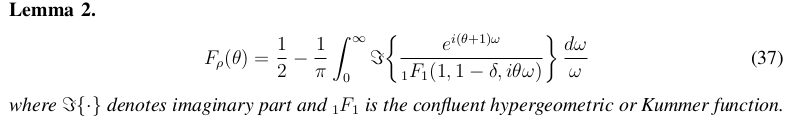
\includegraphics[width=1\linewidth]{123}
\end{figure} \pause
\begin{exampleblock}{Remarque :}
\justify
Dans les expressions analytiques des SIRs, on constate que la connaissance des valeurs de $\rho_k$ détermine entièrement les SIRs. $$SIR_k = N_a \frac{P_k/P}{1+1/\rho_k}$$
\end{exampleblock}
\end{frame}

\begin{frame}
\frametitle{Plan de Présentation }
\begin{enumerate}
	\item \hyperlink{Introduction}{Introduction}
	\item \hyperlink{networkModeling}{Network Modeling}
	\item \hyperlink{conjugateBeamforming}{Conjugate Beamforming}
	\item \hyperlink{spatialDistribution}{Spatial Distribution of $\rho_k$}
	\item \hyperlink{spatialsir}{Spatial SIR Distributions with fixed K}
\end{enumerate}
\end{frame}

\begin{frame}[label=spatialsir]
\frametitle{Spatial SIR Distributions with fixed K}
Dans cette partie on suppose que le nombre d'utilisateurs desservi est fixe.\begin{exampleblock}{Allocation uniforme de puissance :}
\justify
\begin{figure}
	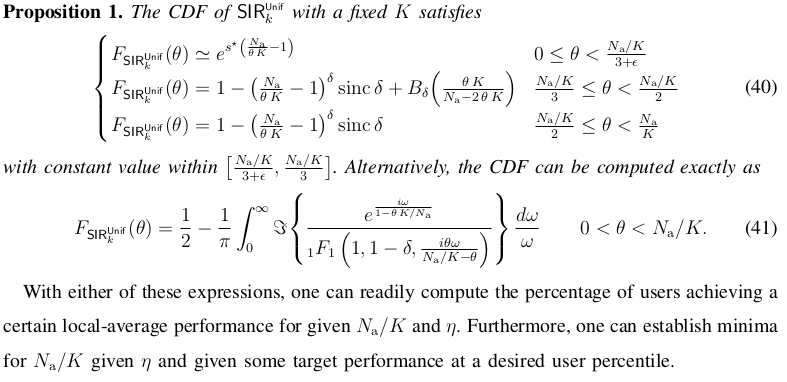
\includegraphics[width=0.7\linewidth]{1}
\end{figure}
\end{exampleblock}
\begin{exampleblock}{Allocation uniforme de SIR moyenne local:}
\justify
\begin{figure}
	
\includegraphics[width=1\linewidth]{2}
\end{figure}
\end{exampleblock}
\end{frame}

\begin{frame}
\frametitle{Plan de Présentation }
\begin{enumerate}
	\item \hyperlink{Introduction}{Introduction}
	\item \hyperlink{networkModeling}{Network Modeling}
	\item \hyperlink{conjugateBeamforming}{Conjugate Beamforming}
	\item \hyperlink{spatialDistribution}{Spatial Distribution of $\rho_k$}
	\item \hyperlink{spatialsir}{Spatial SIR Distributions with fixed K}
	\item \hyperlink{spatialsirk}{Spatial SIR Distributions with Poisson-Distributed K}
\end{enumerate}
\end{frame}

\begin{frame}[label=spatialsirk]
\frametitle{Spatial SIR Distributions with Poisson-Distributed K}
Dans cette partie, on suppose que le nombre d'utilisateurs desservi K suit un processus de poisson. Alors on obtient les résultats suivants : 
\begin{exampleblock}{Allocation uniforme de puissance :}
\justify
\begin{figure}
	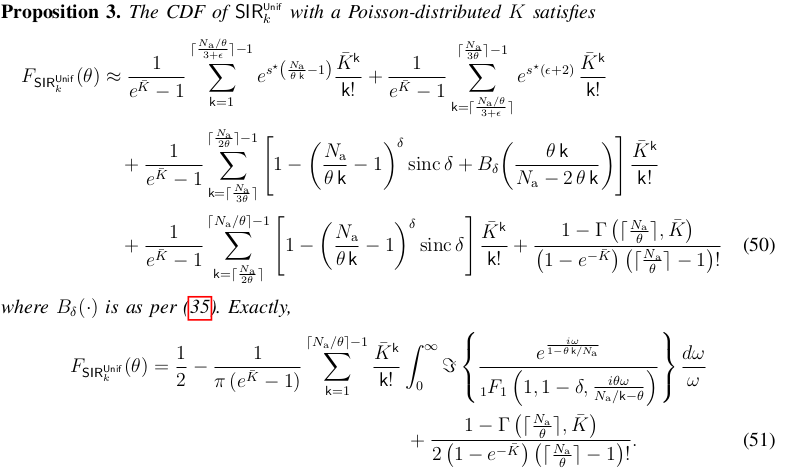
\includegraphics[width=0.8\linewidth]{3}
\end{figure}
\end{exampleblock}
\end{frame}

\begin{frame}
\frametitle{Spatial SIR Distributions with Poisson-Distributed K}
\begin{exampleblock}{Allocation uniforme de SIR moyenne local:}
\justify
\begin{figure}
	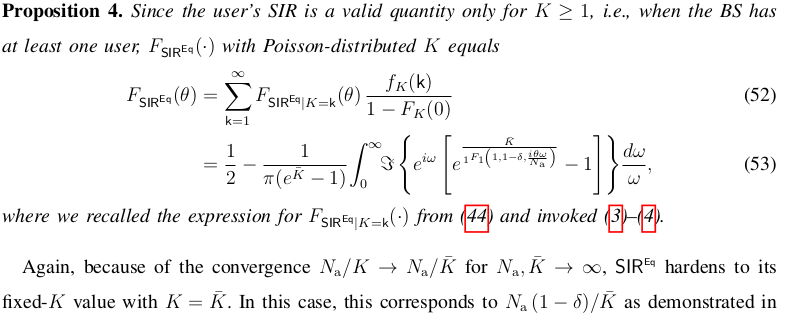
\includegraphics[width=1\linewidth]{4}
\end{figure}
\end{exampleblock}
\end{frame}

\begin{frame}
\frametitle{Plan de Présentation }
\begin{enumerate}
	\item \hyperlink{Introduction}{Introduction}
	\item \hyperlink{networkModeling}{Network Modeling}
	\item \hyperlink{conjugateBeamforming}{Conjugate Beamforming}
	\item \hyperlink{spatialDistribution}{Spatial Distribution of $\rho_k$}
	\item \hyperlink{spatialsir}{Spatial SIR Distributions with fixed K}
	\item \hyperlink{spatialsirk}{Spatial SIR Distributions with Poisson-Distributed K}
	\item \hyperlink{spectralEfficiency}{Spectral Efficiency}
\end{enumerate}
\end{frame}

\begin{frame}[label=spectralEfficiency]
\frametitle{Spectral Efficiency}
\begin{exampleblock}{Efficacité spectrale d'un utilisateur:}
L'efficacité spectrale d'un utilisateur k est donnée par : 
$$C_k = log_2(1+SIR_k)$$
Et sa fonction de répartition vérifie : $$F_{C_k}(x)= F_{SIR_k}(2^x-1)$$
\begin{figure}
	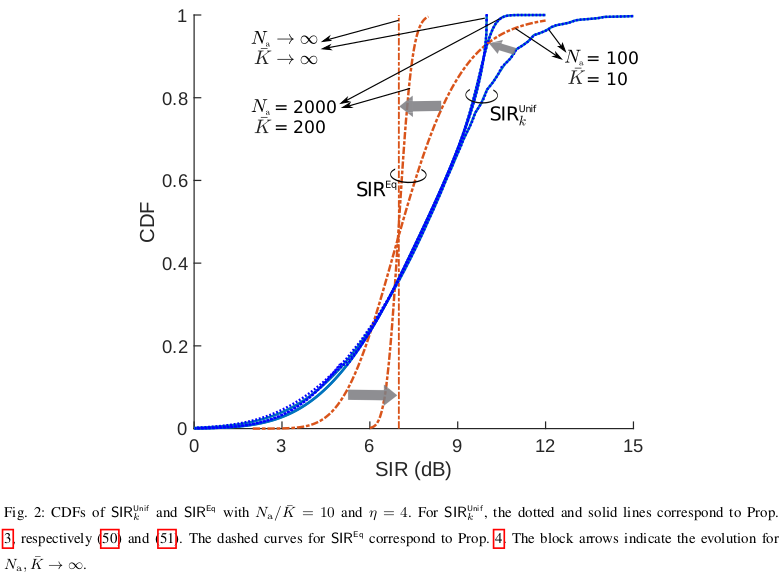
\includegraphics[width=0.5\linewidth]{5}
\end{figure}
\end{exampleblock}
\end{frame}

\begin{frame}[label=spectralEfficiency]
\frametitle{Spectral Efficiency}
\begin{exampleblock}{Efficacité spectrale d'une station de base:}
L'efficacité spectrale d'une BS W est égale à la somme des efficacités spectrales des K utilisateurs servis par cette BS: 
$$C_W = \sum_{k=0}^{K-1}C_k$$
On définit ainsi les efficacités spectrales moyennes des BS et des utilisateurs comme l'espérance des efficacités spectrales : $$\tilde{C}= \mathbb{E}(C_k)$$
$$\tilde{C}_W= \mathbb{E}(C_W)$$
\end{exampleblock}
\end{frame}

\begin{frame}[label=spectralEfficiency]
\frametitle{Spectral Efficiency}
\begin{exampleblock}{Distribution uniforme de puissance:}
Pour une distribution uniforme de puissance et en fixant K, on ontient la proposition ci-dessous : 
\begin{figure}
	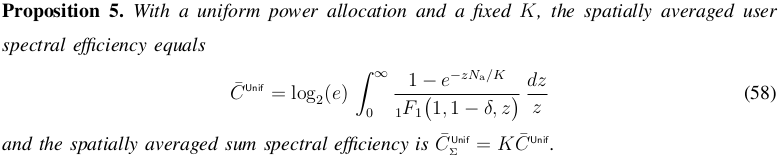
\includegraphics[width=1\linewidth]{6}
\end{figure}
\end{exampleblock}
\end{frame}
\begin{frame}[label=spectralEfficiency]
\frametitle{Spectral Efficiency}
\begin{exampleblock}{Distribution uniforme de SIR:}
Pour une distribution uniforme de SIR entre les utilisateurs et en fixant K, on ontient la proposition ci-dessous : 
\begin{figure}
	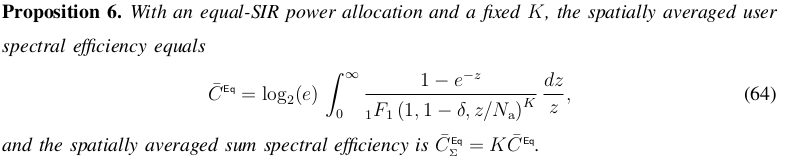
\includegraphics[width=1\linewidth]{7}
\end{figure}
\end{exampleblock}
\end{frame}


\begin{frame}
\frametitle{Plan de Présentation }
\begin{enumerate}
	\item \hyperlink{Introduction}{Introduction}
	\item \hyperlink{networkModeling}{Network Modeling}
	\item \hyperlink{conjugateBeamforming}{Conjugate Beamforming}
	\item \hyperlink{spatialDistribution}{Spatial Distribution of $\rho_k$}
	\item \hyperlink{spatialsir}{Spatial SIR Distributions with fixed K}
	\item \hyperlink{spatialsirk}{Spatial SIR Distributions with Poisson-Distributed K}
	\item \hyperlink{spectralEfficiency}{Spectral Efficiency}
	\item \hyperlink{impactOfNoise}{Impact of Noise}
\end{enumerate}
\end{frame}

\begin{frame}[label=impactOfNoise]
\frametitle{Impact of Noise}
\begin{exampleblock}{Signal-Interference-Plus-Noise}
Les équations écrites précédemment étaient faites en négligeant le bruit ce qui ne reflète pas les conditions de fonctionnement normal. Cependant, on peut constater que le bruit ne va pas modifier de manière significative les équations du SIR avec bruit (SIRN).
\begin{figure}
	\includegraphics[width=0.8\linewidth]{8}
\end{figure}
\end{exampleblock}
\end{frame}

\begin{frame}
\frametitle{Plan de Présentation }
\begin{enumerate}
	\item \hyperlink{Introduction}{Introduction}
	\item \hyperlink{networkModeling}{Network Modeling}
	\item \hyperlink{conjugateBeamforming}{Conjugate Beamforming}
	\item \hyperlink{spatialDistribution}{Spatial Distribution of $\rho_k$}
	\item \hyperlink{spatialsir}{Spatial SIR Distributions with fixed K}
	\item \hyperlink{spatialsirk}{Spatial SIR Distributions with Poisson-Distributed K}
	\item \hyperlink{spectralEfficiency}{Spectral Efficiency}
	\item \hyperlink{impactOfNoise}{Impact of Noise}
	\item \hyperlink{piloteContamination}{Pilot Contamination}
\end{enumerate}
\end{frame}

\begin{frame}[label=piloteContamination]
\frametitle{Pilot Contamination}
\begin{exampleblock}{Signal-Interference-Plus-Noise}
En notant $\mathcal{P}$ l'ensemble des indices des BS réutilisant les pilotes du k ième utilisateur d'intérêt, lorsque l'estimation de canal LMMSE (erreur quadratique minimale linéaire) incorpore la contamination résultante.
\begin{figure}
	\includegraphics[width=1\linewidth]{9}
\end{figure}
\end{exampleblock}
\end{frame}

\begin{frame}
\frametitle{Plan de Présentation }
\begin{enumerate}
	\item \hyperlink{Introduction}{Introduction}
	\item \hyperlink{networkModeling}{Network Modeling}
	\item \hyperlink{conjugateBeamforming}{Conjugate Beamforming}
	\item \hyperlink{spatialDistribution}{Spatial Distribution of $\rho_k$}
	\item \hyperlink{spatialsir}{Spatial SIR Distributions with fixed K}
	\item \hyperlink{spatialsirk}{Spatial SIR Distributions with Poisson-Distributed K}
	\item \hyperlink{spectralEfficiency}{Spectral Efficiency}
	\item \hyperlink{impactOfNoise}{Impact of Noise}
	\item \hyperlink{piloteContamination}{Pilot Contamination}
	\item \hyperlink{autredoc}{Géométrie stochastique et réseaux Massive MIMO}
\end{enumerate}
\end{frame}

\begin{frame}[label=autredoc]
\frametitle{Géométrie stochastique et réseaux Massive MIMO}
\begin{exampleblock}{Autres articles scientifiques}
Il y a d'autres articles scientifiques qui utilisent la puissance de la géométrie stochastique pour la modélisation des réseaux massive MIMO.\\
- On peut notamment citer l'article {\color{blue}{\href{https://www.mdpi.com/2076-3417/10/23/8753}{A Statistical Estimation of 5G Massive MIMONetworks’ Exposure Using Stochastic Geometryin  mmWave Bands}}}  écrit par Maarouf Al Hajj, Shanshan Wang1, Lam Thanh Tu, Soumaya Azzi et Joe Wiart à télécom Paris publié le mois de décembre dernier.\\
- On peut aussi cité l'article {\color{blue}{\href{https://ncrl.seu.edu.cn/_upload/article/files/de/97/92d9b1704b848f2d7cd0ff7d075b/d69642c7-de7d-4486-a75e-462abe9dc56d.pdf}{A Novel Kronecker-Based Stochastic Model forMassive MIMO Channels}}} de Shangbin Wu, Cheng-Xiang Wang, el-Hadi M. Aggoune et Mohammed M. Alwakeel qui utilise une approche de la modélisation stochastique basée sur les modelés stochastiques de Kronecker.

\end{exampleblock}
\end{frame}
\end{document}